\documentclass[9pt,twocolumn,twoside]{pnas-new}
% Use the lineno option to display guide line numbers if required.
% Note that the use of elements such as single-column equations
% may affect the guide line number alignment. 

\templatetype{pnasresearcharticle} % Choose template 
% {pnasresearcharticle} = Template for a two-column research article
% {pnasmathematics} = Template for a one-column mathematics article
% {pnasinvited} = Template for a PNAS invited submission

\usepackage{amsthm}
\usepackage{amsmath}
\DeclareMathOperator*{\argmax}{argmax}

\newtheorem{corollary}{Corollary}
\newtheorem{axiom}{Axiom}
\newtheorem{theorem}{Theorem}
\newtheorem{lemma}[theorem]{Lemma}

\title{A way around the exploration-exploitation dilemma.}

% Use letters for affiliations, numbers to show equal authorship (if applicable) and to indicate the corresponding author
\author[a,1]{Erik J Peterson}
\author[a,b]{Tim Verstynen}
\affil[a]{Department of Psychology}
\affil[b]{Center for the Neural Basis of Cognition, Carnegie Mellon University, Pittsburgh PA}

% Please give the surname of the lead author for the running footer
\leadauthor{Peterson} 

% Please add here a significance statement to explain the relevance of your work
% \significancestatement{TODO}

% Please include corresponding author, author contribution and author declaration information
% \authorcontributions{EJP?.}
\authordeclaration{The authors have no conflicts of interest to declare.}
% \equalauthors{\textsuperscript{1}A.O.(Author One) and A.T. (Author Two) contributed equally to this work (remove if not applicable).}
\correspondingauthor{\textsuperscript{1}To whom correspondence should be addressed. E-mail: Erik.Exists@gmail.com}

% Keywords are not mandatory, but authors are strongly encouraged to provide them. If provided, please include two to five keywords, separated by the pipe symbol, e.g:
% \keywords{Keyword 1 $|$ Keyword 2 $|$ Keyword 3 $|$ ...} 

\begin{abstract}
The exploration-exploitation dilemma is considered a fundamental problem in the learning and decision sciences. Exploitation means simply choosing most valuable option. Exploration in the dilemma means searching for unknown rewards. The intrinsic uncertainty (or partial observability) of this search makes the problem mathematically intractable. Focusing only on rewards though ignores the direct certain value of exploratory behavior: the acquisition of general information about the world. Here, we challenge the traditional approach to the dilemma and offer an alternative account based in information theory. We first derive an axiomatic measure of information value. We use this to decompose the exploration-exploitation dilemma into a tractable two-part problem, creating separate mathematical objectives for exploration and exploitation. From this we derive a new learning policy which we prove is certain to optimally explore, maximize total information value, and maximize total rewards. In simulation, we show how this policy generates naturalistic behavior in both simple and complex simulated worlds. 

% Finally we who how this same theory predicts exploratory actions of \textit{EVERY FUCKING LIVING THING?!}. % TODO....
\end{abstract}

% \dates{This manuscript was compiled on \today}
% \doi{\url{www.pnas.org/cgi/doi/10.1073/pnas.XXXXXXXXXX}}

\begin{document}
\verticaladjustment{-2pt}
\maketitle

\thispagestyle{firststyle}
\ifthenelse{\boolean{shortarticle}}{\ifthenelse{\boolean{singlecolumn}}{\abscontentformatted}{\abscontent}}{}
Why do animals explore? We know animals will explore when there are no rewards present, or expected \cite{TODO}. This suggests they simply wish to better understand their world. Animals also explore as play, trying to understand other agents \cite{TODO}, to learn strategies \cite{TODO}, and to refine their actions repertoires \cite{TODO}. In a more classical sense animals also explore to find more food, water or mates. In a general sense then it seems animals explore to gain information \textit{and} to acquire more rewards.

When an animal explores looking for greater rewards there is a often a trade-off to be made with choosing more conservative actions, likely to produce desirable results (what we call exploitation) \cite{TODO}. The optimal policy for exploitation is well known. One calculates total expected future rewards \cite{TODO}. The optimal policy for exploration, on the other theoretical hand, remains elusive \citep{thrun1992active, dayan1996exploration, findling2018computational, gershman2018deconstructing}. 

Exploration for reward is often reframed as a problem of ``information seeking'', that is implemented through the use of motivational bonuses on less frequently used actions \citep{Sutton1990, dayan1996exploration}, or information is modeled as the internal isomorphism of a tangible, external reward (a so-called \textit{intrinsic reward}). However by linking the value of information to rewards, the problem of optimal exploration remains mathematically intractable \citep{thrun1992active, dayan1996exploration, findling2018computational, gershman2018deconstructing}. 

Here we propose an alternative view: \textit{Information is valuable for its own sake}. We argue two points. One, an animal should seek to maximize information just as vigorously as reward. Two, the two goal of maximizing information is entirely separate from goal of maximizing rewards. 

Our contributions are threefold. We first use axiomatic information theory to create a new general measure of information value. Next we develop a new theory for exploration that optimally maximizes information value. This theory is purely deterministic, meaning exploration no longer relies on random sampling and is instead perfectly rational. Finally, we show how the exploitation-exploitation dilemma can be formally redefined using two objectives, maximizing information value \textit{and} maximizing reward value. From this view we derive a new learning theory which allows for simultaneously optimal and deterministic solutions to \textit{both} the problems of exploration and exploitation.

\section*{Results}
To make up for any ``missed'' rewards during exploration information treated as a fictive reward signal.  When this happens the information term is generally weighted, and added to any natural rewards leading (as seen in Eq.~\ref{eq:total_r_I}). 

To denote information we use a generic term $I$ to stand in for a pack of theoretical possibilities, including novelty bonuses, curiosity signals, entropy terms\cite{TODO}. The classic, or natural, reward is denoted by $r$, and $\beta$ is used for the weight. For convenience, we confine confined rewards to be a binary variable, and $I$ to the real numbers ($r \in 1{0, 11}, I \in \mathbb{R}, \beta > 0$). When no information is included, the problem of estimating optimal total value $V^{*}_{pi_R}$ reduces to Eq.~\ref{eq:total_r} for a set of states $S$ and finite time $T$.

\begin{equation}
    V^{*}_{pi_R} = \sum_{t \in T, s \in S} r
    \label{eq:total_r}
\end{equation}

\begin{equation}
    V^{*}_{pi_R} = \sum_{t \in T, s \in S} r + \beta I
    \label{eq:total_r_I}
\end{equation}

During exploration rate of rewards $\frac{dr/dt}$ can decline, for a time. If there is no $\beta I$ term, then value declines (Eq~\ref{eq:total_r}). This decline is the heart of the trade-off. Adding an information term can numerically balance out losses, ensuring the animal chooses to explore. 

Rebalancing reward with information seems at the surface simple and intuitive. But it also comes with a cost. If the goal is to maximize $r$, as it is by define in the dilemma problem, adding a fictive reward obscures this aim while offering no guarantee of a performance increase. After all, an increase in $V$ can come from a $r$ or from the fictive $\beta I$. Put another way, $\beta I$ can drive exploration but can't help with the fundamental dilemma problem which is really about Eq~\ref{eq:total_r}.

Here we suggest a new view: \textit{information is valuable for its own sake}. 

Animal's learn and explore the world for a range of reasons \cite{TODO LIST FROM INTRO}. Theory should take this into account. Specifically, we study a case with independent policies. One policy to maximize reward ($\pi_R$, Eq.~\ref{eq:total_r_2}) and one for information value ($\pi_E$, Eq.\ref{eq:total_e}). As well see in coming sections, separating the variables allows for exploration without obscuring the ability to optimize rewards. It also let's us offer theoretical guarantees for exploration quality, rooted in dynamic programming.

\begin{equation}
    V^{*}_{pi_R} = \sum_{t \in T, s \in S} r
    \label{eq:total_r_2}
\end{equation}

\begin{equation}
    V^{*}_{pi_E} = \sum_{t \in T, s \in S} I
    \label{eq:total_e}
\end{equation}

\subsection*{Information is not a reward}
Besides the empirical and computational case made above, a first principle analysis of information and reward shows they have opposing properties:

\begin{enumerate}
    \item Rewards are a conserved resource. Information is not. 
    \item The same kind of reward can be consumed many times without necessarily losing value\footnote{In practice, there are satiety effects but these are not a necessary part of the reward's value}. Information once learned has no value in being be learned again.
\end{enumerate}

These can be seen more intuitively by example. In \texit{1.}, If a rat shares its potato chip with a cage-mate, it has less food for itself. Compare that chip to a new idea. Explaining a new idea to lab-mate does not require forgetting the idea yourself. In fact, it's often the opposite.

In \texit{2.}, eating one potato chip often means wanting another. Where as if you know the capital of the United States, there is no value in being told the capital of the United States is Washington DC.

These philosophical differences lead to mathematical ones. To evenly share a reward $r$ between $n$ others, $r_n = \frac{r}{n}$. Where as for information value can in principle be shared without loss, $I_n = I$. Likewise, if an animal is learning about some state of world $s$ the value of information about $s$ should decrease with time. Assuming learning can asymptote, then as $t \rightarrow \infty, I_s \rightarrow 0$. For rewards, value never changes. So as $t \rightarrow \infty, r_s \rightarrow r_s$. Though, including reward satiety effects may somewhat diminish $r_s$.

For empirical, philosophical, and mathematical reasons we've suggested reward and information should be optimized separately. To make this suggestion formal in the next sections we \begin{enumerate*} \item derive a general measure information value using an axiomatic approach, \item derive a deterministic optimal policy to maximize this measure, and \item derive a new optimal learning rule which can simultaneously maximize information \textit{and} reward value \end{enumerate*}. We also show how efficient coding can lead to efficient re-exploration in environments that change with time. 

    
% ---------------------------------------------------------------------------
\subsection*{If information is not a reward, how can we value it?}
Shannon originally developed information theory without any sense of what information ``means''. He focused on simply transmitting symbols. To work the theory does need to know what those symbols refer to, and is therefore extremely general \citep{Shannon1948}. Many attempts have since been made to instill information theory with meaning \citep{Kolchinsky2018}, and with meaning value follows. Most of these attempts require a ``salience'', or ``relevance'', or ``training'' signal (where all three terms amount to near the same thing), while others have taken an evolutionary approach \citep{Kolchinsky2018}.  
% TODO bump up refs

Instead of trying to define meaning more broadly, we take an axiomatic approach to define value: \textit{listing key properties (axioms) that any naturalistic measure of information value should have, and arrive a metric that satisfies these}. Put another way, we suggest information value can be strictly internal to an agent, but that meaning requires an explicit outside reference. This purely self-referential approach to information value is extremely general for the same reasons as Shannon's original theory. We only compare distributions, and do not consider what those distributions refer to.

We begin formalizing information value with five axioms:

\begin{axiom}
    The value of information about some event $x$ depends \textit{only} on what is already known about $x$ (and not $x$ itself).    
    \label{ax:1}
\end{axiom}
\begin{axiom}
    Information about some event $x$ that is known with no uncertain has a value of exactly 0.
    \label{ax:2}
\end{axiom}
\begin{axiom}
    The value of information about some event $x$ is non-negative. 
    \label{ax:3}
\end{axiom}
\begin{axiom}
    The value of information of information about some event $x$ should be be higher when its uncertainty increases $p(x)$ compared to when it decreases.
    \label{ax:4}
\end{axiom}
\begin{axiom}
    For a some set of events $X$, specific (or localized) changes to the local structure of the distribution $p(X)$ uncertainty are more valuable than global changes.
    \label{ax:5}
\end{axiom}

Axiom~\ref{ax:1} closes value calculations over the agent making them. Informally, we capture the idea that ``subjective value depends only on the subject's own experience''.  In Axiom~\ref{ax:2} we capture the idea that, ``if you know something \texit{perfectly), there is no value in learning it again''. Axiom~\ref{ax:3} exists to impose that idea that, ``learning new information is always good, in principle''. In practice, of course, learning some new information can have undesirable consequences. But any these consequences are not part of the information itself, but live in its use. Axiom~\ref{ax:4} ensures information value tracks risk to animals surviving in the natural world, ``it's more valuable to know about an increase in uncertainty than an increase in certainty''. Axiom~\ref{ax:5} covers the precept that, ``specific information is more valuable than general information.'' 

Here, we satisfy these Axioms using ideas from information theory. Our choice of the KL divergence (below) is not as far as we are aware a unique information theoretic solution; it's simply a satisfactory choice. 

% ---------------------------------------------------------------------------
\subsubsection*{Using the KL divergence.}
Calculations in information theory are done over probability distributions $p(.)$, on some set of symbols $S$. Here, symbols are states of the world (a notion we fully formalize below). 

\begin{definition}
    We call a distribution over a set of states of the world $S$ a \textit{memory distribution} and denote it with $M$, where $M(s) = p(s), \ \text{where} s \in S$.    
\end{definition}

The Kullback--Leibler divergence satisfies all five value axioms (Eq.~\ref{eq:KL}). 

\begin{equation}
    KL(M', M) = \sum_{s \in S} M'(s) \text{log} \frac{M'(x)}{M(x)} 
    \label{eq:KL}
\end{equation}

\begin{definition}
    Let $E$ represent value of information, such that $E = KL(M', M)$ (Eq.~\ref{eq:KL}), where $M$ is some initial memory and $M'$ is an update memory after observing some state $s'$.
\end{definition}

Axiom~\ref{ax:1} is satisfied by limiting $E$ calculations to successive memories. Axiom~\ref{ax:2}-\ref{ax:2} are naturally satisfied by using KL. That is, $E = 0$ if and only if $M' = M$ and $E \geq 0$ for all pairs $(M, M')$. Likewise, KL is naturally monotonic to overall changes in probability by its log-likelihood ratio term, $log \frac{M'(x)}{M(x)}$. This satisfies Axiom~\ref{ax:4}. 


To make Axioms 4-5 more intuitive, in Figures~\ref{fig:metrics_updown}-\ref{fig:metrics_specifity} we show how KL changes between an initial distribution (always shown in grey) and a variety of ``learned'' distribution (colored). For simplicity's sake we use a simple discrete distribution, representing the likelihood of the first four non-negative integers $(0,1,2,3)$. Though the illustrated patterns should hold true for any pair of distributions.

Axiom~\ref{ax:4} can be seen at work in Figures~\ref{fig:metrics_likelihood}. and \ref{fig:metrics_specifity}. In Figure~\ref{fig:metrics_specifity} we see KL increases substantially more, for a the same local increase in probability, when that increase comes with a localized decrease, rather than with an even re-normalization. Thus in this example, the KL divergence exhibits the required sensitivity to local structural changes in probability distribution.

\begin{figure}
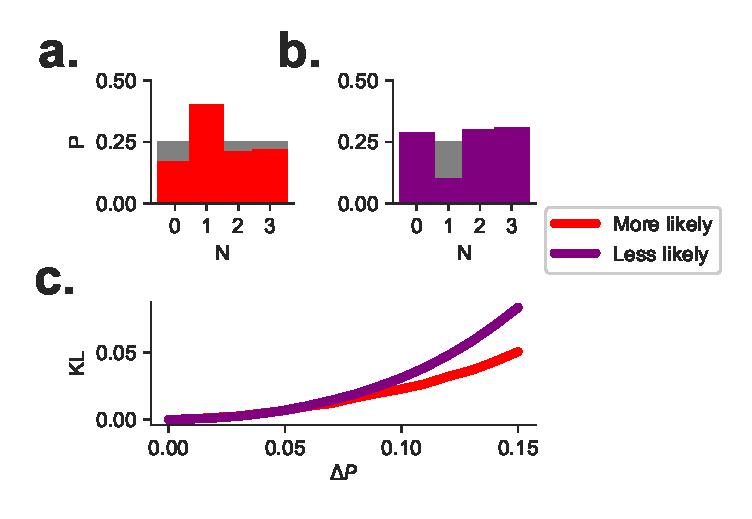
\includegraphics[width=0.4\textwidth]{figures/metrics_likelihood.eps}
\caption{
\textit{Uncertainty and information value.
\textbf{a.} Increasing probability (red) compared to uniform (or maximum entropy) distribution (grey).
\textbf{b.} Decreasing probability (purple).
\textbf{c.} The change in KL as the probability density changes from the reference (grey), either increasing or decreasing the likelihood of a ``1'' appearing.}}
\label{fig:metrics_likelihood}
\end{figure}

\begin{figure}
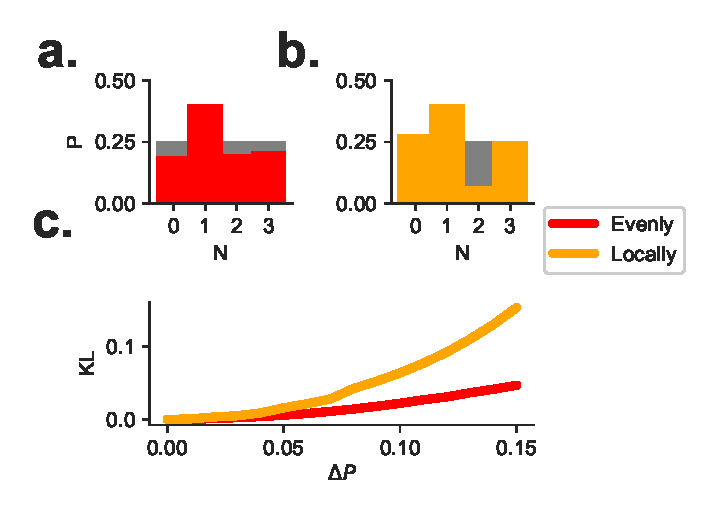
\includegraphics[width=0.4\textwidth]{figures/metrics_specifity.eps}
\caption{
\textit{Local probability structure and information value. Both distribution shown in a. and b. have the same total increase in the probability of a ``1'' appearing.
For \textbf{a.}  the necessary corresponding decrease in probabilities for all numbers (0, 2, 3) is evenly redistributed.
In \textbf{b.} the loss is focused locally on ``2''. 
\textbf{c.} The KL divergence increases more rapidly for local changes in probability density}}
\label{fig:metrics_specifity}
\end{figure}

To a skeptical reader, Axioms~\ref{ax:4} and~\ref{ax:5} may seem unnecessary. A simpler natural set of Axioms is to keep 1-3 but replace 4-5 with a new axiom that only requires information value track the total changes in probability flux with each new state observations, meaning $\text{E \sim \frac{dM}{ds}$. We considered this, but rejected it for two reasons. Axiom~\ref{ax:4} arose from the substantial experimental literature showing how animals are more sensitive to decreases in uncertainty \cite{TODO}. Our motivation for Axiom 5, was different and mostly intuitive. We found it inescapable as theorists and scientists to not favor more specific, therefore more actionable, information. 

Still, the skeptical reader may be unconvinced and would hope for a simpler set. For them, we can report that the derivative $E = |frac{dM}{ds}|$ can be used in place of our Axioms~\ref{ax:4}-~\ref{ax:5}, and Theorems~\ref{TODO} re-proven with trivial changes.

% ---------------------------------------------------------------------------
\subsection*{Finding the optimal policy}
% Intro - the state space, E, and R. Max E. 
% Show the formalism, gentle like.
% Optimal substruture. E max as dynamic programming problem
% Bellman form
To derive an optimal policy for maximizing information value we borrow some formalisms from reinforcement learning, and it's parent dynamic programming. We say an agent occupies a state $s$, which in practice can be a simple as their position in the world, the current visual input, or any other combination of sense information. To keep the theory tractable, we assume that the total number of states an animal might visit $S$ is finite. Formally, $s\ in \textbf{S}; \textbf{S} \in \mathbb{R}^N$, where we use real numbers to represent states and $N$ is the total number of states. We also limit the number of actions $a$ animal might take to finite real set, $a \in \textbf{A}; \textbf{A} \in \mathbb{R}^K$, where there are $K$ actions. 

When deciding what action to take, we say an that animal consults its policy function, $\pi$. Formally, we let $\pi$ be a policy function that maps a state $s$ to an action $a$, $\pi : s \rightarrow a$, such that $s \in S, a \in A$.

How an animal acts on the world, and how the environment responds, is in reality complex and depends on a lot of local context. % TODO make this an exmample or more concrete....
 We abstract over this detail and assert there exists a transition function $\Lambda$ which combines the current state $s$ and an action $a$ to generate some new state $s'$. Formally, let $\Lambda$ be a transition function which maps a $(s,a)$ 2-tuple to a new state $s'$, $\Lambda : (s, a) \rightarrow s'$. 

A policy function and transition function combine to generate a path $P$, finite ordered collections of states $s$, such that $s \in S$ and the length of $T = |P|$ where we use $t$ to index into $P$. A path $P$ can also be defined recursivly as, $P(t+1) \leftarrow \Lambda(P(t), \pi(P(t)))$.

Learned information is said to be stored in a finite perfect (i.e., noiseless) memory, denoted by $\textbf{M}$. As $M$ is probability distribution, we let $M$ be a table of independent states $S$ and actions $A$, such that $M \in (0, 1)^{N\text{x}K}$. % TODO: Do I need to formalize independent somehow?

The memory $M$ is update with a loss function $L$, subject to $min_a L(M, {s})$. Formally, let $L$ be a memory function that maps a memory $M$ into itself, given some observed state $s$, $L : s, M \rightarrow M$. 


\textit{With a loss of generality}, we assume that $L(.)$ is convex, and that every observation $s$ leads to learning progress unless $L(s) = 0$. That is, the gradient of $L$ is, $\frac{dL_{\pi_{a}}}{ds} \leq 0$ for all $s \in P$. These are strong statements on the animal's ability to learn from it's world. They allow us to develop several critical theorems, but might seem overly restrictive.

We discuss our measure of information value $E$ in detail above. But for completeness, let $E$ be the information value between two successive memories, $M$ and $M'$ corresponding to states $s$ and $s'$, defined by the KL divergence so $E(s) := KL(L(s, M), M) = KL(M', M) = \sum_{s \in S} M'(s) \text{log} `\frac{M'(s)}{M(s)} $. 

Our formalism for information value yields a non-zero positive number with every new observation $s'$, unless learning has already converged. This allows us to consider the problem of maximizing $E$ from a purely iterative point of view, i.e. dynamic programming. There is no need for trying to solve the protracted credit assignment often needed in reinforcement learning.

\texit{Note}: when discussing value optimization in general, and the exploration-exploitation dilemma in particular, it is standard to embed the learning problem in a Markov decision space. In this space, each transition is independent of the history of transitions, and that each each yields a value $V$ or reward $R$, where $R$ or $V$ are not dependent on the state of the agent itself. Our definition of information value $E$ violates both these formalisms. However the information value is calculated piece-wise, iteratively, between observations, which leaves open the possibility of finding an optimal iterative learning rule. 

\begin{theorem}
    Assuming a independent state memory $M$ and a value function $E$, a path $P$ has optimal substructure for a optimal policy $\pi_E$.
\end{theorem}
\begin{proof}
    Assume path $P$ has an optimal value $V_{\pi_E^*} = sum^t_P \gamma KL(L(M, P(t)), M)$ for policy $\pi_E$, and that subproblem $\hat P$, who's optimality we wish to test, contains every state up until the last one, $t$. 
    
    Let $\hat P = P - s_t$, and $\hat V' = V - E_t$.

    For the sake of contradiction assume there exists an alternative policy $\pi_E^*$ that gives a path $\hat P^* \neq \hat P$ and for which $\hat V^* > \hat V$. 

    To recover the known optimal path $P$ we learn about the final observation $s_t$, giving $P^* \neq P$ and $V* > V$ which contradicts the purported optimality of $V$.
\end{proof}

The value function of the optimal value function is $V_{\pi_E^*} = sum^t_P \gamma KL(L(M, P(t)), M)$. 

Having established the optimal substructure of $P$, for an independent memory $M$ and value function $E$, we can use Bellmans' equation in the standard way to derive an optimal greedy iterative policy:

\begin{align}
    V(s_t) = F(s_t, a_t) + \gamma max_{a \in A} F(s_{t+1}, a_{t+1}) \\
    V(s_t) = F(s_t, a_t) + \gamma max_{a \in A} F(\Lambda(s_t, \pi(s_t)), \pi(s_t))
\end{align}


% ---------------------------------------------------------------------------
\subsubsection*{Optimal exploration}
A policy that maximizes information value should also do a good job exploring. It would be ideal if the exploration pattern was also optimal, for some useful definition of optimal. But there is no agreed upon definition of optimal exploration because, as we discussed in the introduction, exploration is an intractable problem when framed in terms of reward seeking. 

There are many intuitive options when trying to construct a general definition for exploration. For example, different definitions might require all states are explored in the fixed number of steps, or with the least effort, or that while exploration is ordered to also maximize rewards. Rather than try and argue for one or another view, we suggest a \textit{minimal definition for optimal exploration} which that satisfies two criteria for finite environments. 

\begin{enumerate}[noitemsep,wide=0pt,leftmargin=\dimexpr\labelwidth+2\labelsep\relax]
    \item Optimal exploration should visit all states of the environment at least once. 
    \item Exploration should cease, but \textit{only} once learning about the environment has plateaued. 
\end{enumerate}

Criterion 1 seems to be required as it's converse is absurd: an exploration which lest some states unseen can hardly be considered complete, and therefore optimal.

Criterion 2 might at first seem unnecessary; Exploration, by definition, seeks the unknown. So it does not necessarily need to terminate. If the environment changes too fast, the agent has a limited memory or has no memory at all, the optimal choice would be endless exploration. If, however, the environment is learnable and stationary, then an optimal exploration policy should cease once the environment is learned to some criterion (which we formalize below). That is, exploration is redundant if there is nothing new to learn.

For brevity we will refer to our minimal definition as \textit{optimal exploration} and use $\pi_E$ to denote any action policy which satisfies this definition.

While on the surface simple, our minimal criterion for exploration is not \texit{guaranteed} to be satisfied by any existing approach. Specifically, criterion 2 is not satisfied. (Criterion 1 can be satisfied by nearly any random policy given a sufficiently long time to explore.) % TODO more on this. How do epsilon, softmax, H max, all fail..


% ---------------------------------------------------------------------------
\subsubsection*{Greedy exploration} 
Here we prove that policy which strictly maximizes information value can also guarantee optimal exploration. 

Informally stated, to achieve optimal exploration an agent should \textit{try and learn everything possible} and, \textit{when there is nothing to learn, do nothing}. Using our definition of information value (Eq. \ref{eq:KL}) we formalize these as:

\begin{enumerate}[noitemsep,wide=0pt,leftmargin=\dimexpr\labelwidth+2\labelsep\relax]
    \item The goal of any agent is to learn an action policy $\pi$ that maximizes total information value, $\argmax_{\pi_E} \ \sum_X \sum_T E$, over all states $x \in X$ and times $t \in T$, for some environment $X$.
    \item If information value converges to zero, then the action policy should approach some null or default action policy. That is, $\sum_X E = 0$, \ $\pi \rightarrow \O$ or a slightly less strict form that allows for imperfect learning, $\sum_X E < \epsilon $, \ $\pi \rightarrow \O$, where $\O$ represents rest or another default action policy (e.g., grooming or checking Facebook).
\end{enumerate}

Using the Bellman equation we derive a learning rule $J_E$ and a \textit{deterministic} action policy $\pi_E$, over a set of $T$ observations and environment $X$, that \textbf{(1)} provably converges on a policy that maximizes total information value (i.e., $\argmax_{\pi_E} \ \sum_X \sum_T E$) and \textbf{(2)} converges to optimal exploration (i.e., $\pi_E \rightarrow \pi^*$).

To test for satisfaction of criterion 2 in our definition of optimal exploration we introduce a set $Z$. Let $Z$ be set of all visited states, where $Z_0$ is the empty set $\{\}$ and $Z$ is built iteratively, over a path $P$, such that $Z = \{s | s \in P \text{and} s \not\in Z\}$.

\begin{theorem}{Optimal exploration (uniqueness)}
A greedy policy $\pi$ is the only deterministic policy which ensures all states in $S$ are visited, such that $Z = S$.
\end{theorem}

 % TODO is this structured right? Lemmas and all?
\begin{proof}
    \textbf{Definition}: 
    \begin{align}
        a \leq b \Leftrightarrow \exists c; b = a + c \\
        a > b \leftrightarrow (a \neq b) \wedge (b \leq a) 
    \end{align}

    \begin{lemma}
    Let $\textbf{E} = (E_1, E_2, ...)$ be ranked series of $E$ values for all states $S$, such that $(E_1 \geq E_2, \geq ...)$. To swap any pair of values ($E_i$ \geq $E_j$) so ($E_i$ \leq $E_j$) be definition $E_i - c = E_j$.  

    \textbf{Recall}: $\delta E(s) < 0$ 

    Therefore, $\exists \int \delta E(s) \rightarrow -c$. 
    \end{lemma}

    \begin{lemma}
    Conversely, if we wish to swap ($E_i$ \leq $E_j$) so ($E_i$ \geq $E_j$) by definition $\not \exists c; E_i + c = E_j$, as $\not \exists \int \delta E(s) \rightarrow c$. 
    \end{lemma}

    % TODO This is too loose.
    To complete the direct proof, assume that some policy $pi^* \neq pi$. The policy $\pi^*$ must choose between $k$th best options, eventually after $T$ the $k$ options will be 0, but by Lemma TODO the top $k-1$ are inaccessible. Therefore, $pi^* \rightarrow Z /neq S$.
\end{proof}

\begin{theorem}{Optimal exploration (convergence)}
    A deterministic greedy policy $\pi$ will resample $S$ until convergence at $\sum_{s \in S} E < \epsilon$.
\end{theorem}
\begin{proof}
    In theorem TODO, it was proven that deterministic greedy policy will visit each state in $S$ over $T$ trials, unless $\sum_{s \in S} E < \epsilon$. 
    
    If we assume that over $T + \delta T$ that $\sum_{s \in S} E > \epsilon$ a deterministic greedy will then revisit each state over other interval $T + \delta T$. By induction then, for any later interval $\delta T$ a deterministic greedy policy will revisit all states until (by definition) $\sum_{s \in S} E < \epsilon$.
\end{proof}

Exploration is often considered to be a stochastic process. An animal makes a weighted random choice to try and maximize rewards in the long term. We've shown here that from the point of view of information value, a noisy policy would be suboptimal; a deterministic greedy policy is optimal.

We conjecture that a greedy $E$ policy also leads to the minimal possible number of samplings strategy for any convex loss function $L$. We prove this in the limited case of a ``perfect'' one-shot learning system.

% TODO: one shot proof

% ---------------------------------------------------------------------------
\subsection*{A way around the dilemma} \label{sec:Obj1b}
So far we've shown that for an independent memory $M$ there exists an optimal deterministic learning policy to maximize information value $E$, that that this same learning rule exhibits optimal exploration over a finite number of states. 

Here we derive new meta-policy $\pi_{\pi}$ that can simultaneously exhibit optimal maximization of information value, show optimal exploration, and also optimally maximize rewards (over an infinite time horizon).

Several known optimal policies for reward learning are known, many using an infinite time horizon. We refer to this family of learning rules in abstract by $\pi_R$

By confining rewards to the typical binary set ${0, 1}$ and by assuming rewards are stochastic, constrained by $p(R = 1) < 1, \all s \in S$, we can build on Theorems TODO to derive a deterministic \texit{meta-greedy} policy $\pi_{\pi}$ which ensures optimal returns for information value, reward value, and that achieves minimally optimal exploration.

\begin{equation}
    \pi_{\pi} = \left\{
      \begin{array}{lrc}
        \pi_E & : E_t - \epsilon > R_t \\
        \pi_R & : R_t \geq E_t - epsilon \\
      \end{array}
    \right
    \label{eq:meta_greedy}
\end{equation}

\begin{theorem}
    Assuming an infinite horizon, a memory $M$ (Def. TODO), a value function $1 > E \ge 0$ (Eq.~\ref{eq:KL}) and $R\ in \{0, 1\}. p(R = 1) < 1, \all s \in S$, the \textit{meta-greedy} policy $\pi_{\pi}$ (Eq.\ref{eq:meta_greedy}), optimally maximizes total information value if $\pi_E$ is itself optimal, has optimal exploration if $\pi_E$ is greedy, and optimally maximizes total reward if $pi_R$ is itself optimal.
\end{theorem}
\begin{proof}
    \textbf{Recall}: in Theorem TODO we prove the optimality of $\pi_E$.
    \textbf{Recall}: we assume $\pi_R$ has some proven optimality.

    The optimality of $|\pi_{\pi}$ can be seen by direct inspection. If, $p(R = 1) < 1$ and we have an infinite horizon, the $pi_E$ will have a unbounded number of trials meaning the optimally of $P^*$ holds. Likewise, $\sum E < \epsilon$ as $T \rightarrow \infty$, ensuring $pi_R$ will dominate $\pi_{\pi}$ therefore $pi_R$ will asymptotically converge to optimal behavior.
\end{proof}

In proving the total optimality of $\pi_{\pi}$ we limit the probability of a positive reward to less than one, denoted by $p(R = 1) < 1$. Without this constraint the reward policy $\pi_R$ would always dominate $\pi_{\pi}$, limiting information maximization and exploration to suboptimal levels. An alternate way to handle the edge case $p(R = 1) = 1$ would be to introduce the a model of reward satiety, where reward value decays asymptotically with repeated exposure. % TODO example of satiety with math.

% TODO: talk about the dynamics more intuitively. The less likely R the more exploration, until convergence.

While successfully maximizing $E$ leads to $\bar E \rightarrow 0$ (as explained in Section~\ref{sec:Obj1a}). The differing asymptotes suggest that each policy $\pi_E$ and $\pi_R$ should be learned separately, and they could usefully compete for control of the agent at any given moment in time $t$. We call this \textit{meta-greedy learning}.

We continue to restrict $\pi_E$ to be deterministic. We also now restrict $\pi_R$ to be deterministic, leading to a unique conception of the exploration-exploitation problem: an initial value problem. 

For every state $s$ the algorithm chooses an action $a \sim \pi_{\pi}(s)$, leading to a new state $s'$ by $\Lambda(s, a)$ and a (possible) reward $r \in \{0,1\}$. In this arrangement both $\pi_E$ and $\pi_R$ are updated by their respective learning rules with each transition set $(s, a, s', r)$. That is, learning can be done in parallel, making it cooperative, but action control is adversarial governed by the inequality in Eq~\ref{eq:meta_greedy}.

\section{Discussion}

\subsection*{The assumptions on learning and memory}.
\subsubsection{Non-convex learning}
We justify our constraints on $L$ in two ways. First, assuming convexity is common tactic used to make learning proofs tractable. Second, we argue that the value of information is only \textit{certainly useful} when an agent can learn about it's world. If learning begins to diverge, $\frac{dL_{\pi_{a}}}{ds} > 0$) $E(s, a)$ must also grow (see Eq~TODO). If noise or stimulus complexity drove a momentary loss of learning progress, this drive will lead the agent to ``resample'' these stimuli which max return $L$ to a negative trajectory. In this case, maximizing $E$ remains a sound objective. On the other hand, if $L$ diverged due a problem with the learning algorithm itself, say a bad seed in a deep reinforcement learning model, then maximizing $E$ may exacerbate the problem leading to a potentially catastrophic feedback loop. In this case maximizing $E$ seems unsound, though it is not clear if any action policy would be better unless that is the agent has access to it's own learning rule allowing it to self-diagnosis the problem.

% TODO: keep this? drop this?
\begin{theorem}
    The assumption $\frac{dL_{\pi_{a}}}{ds} \leq 0$, can be replaced with $\mathbb{E} [\frac{dL_{\pi_{a}}}{ds} \leq 0]$ over an infinite time horizon, with an increase in generality.
\end{theorem}
\begin{proof}
....
\end{proof}


\subsubsection*{Dependent states}.
....


\subsection*{Curiosity and value}.
% TODO section on curiosity:

A skeptical reader would suggest we're swapping an accepted term \textit{curiosity}, with another \textit{information value}. We acknowledge this, and have wondered it ourselves! It's that intuitively, curiosity often seems to dim more quickly than certain knowledge reaches its full brightness. That is, learning needs more than curiosity. Learned information has to have its own independent value. This is, in the end, why we formalize the value of information using simple axions. 

\subsection*{Learning structure and value}.
We've explored only a simple memory model. 

.... Bayes, trajectories, and other model building.

By redefining the problem of exploration and in defining the value axioms, which we known have multiple possible solutions, we offer a way to these methods for model-building and fold them seamlessly and optimally into a value optimization framework. 

\bibliography{library}
\end{document}

    
% ----------------------------------------------------------------------------
% ----------------------------------------------------------------------------
% ----------------------------------------------------------------------------
% ARCHIVE - prior to maxent reformulation on 11/28
% ----------------------------------------------------------------------------
% ----------------------------------------------------------------------------
% ----------------------------------------------------------------------------

% Exploration is about decreasing uncertainty. Valuing exploration is about increasing uncertainty.

% Info games as max ent?


% The first expression which comes to mind as a candidate to satisfy these is, of course, Shannon entropy $H$.

% \begin{equation}
%     H(X) = -\sum_{i=1}^{N}p(x_i)\ I(x_i)
% \end{equation}

% Where

% \begin{equation}
%     I(x_i) = \text{log}\ p(x_i) 
% \end{equation}

% But entropy doesn't meet the requirements. $H$ declines once $p < 0.5$. 

% The negative surprise term $-I$ though is good candidate to satisfy $1$ and $2$: As $p(x_i) \rightarrow 1$, then $-I$ declines. Conversely, $-I$ grows as $p(x_i) \rightarrow 0$.

% Axiom $3$ is satisfied making surprise relative, and taking the difference between two sets of observations, old $X$ and new $X'$. 

% \begin{equation}
%     \label{eq:M1}
%     M = I(X) - I(X')
% \end{equation}

% When $X' \not \in X$, $M$ simplifies to simply

% \begin{equation}
%     \label{eq:M2}
%     M = -\text{log}\ p(x')
% \end{equation}

% While if $X'$ is the same as $X$, then all the terms in Eq.~\ref{eq:M1} cancel and $M = 0$. $M$ grows both as $x'$ becomes less likely, and as it differs from what is already known in $X$.

% This simple definition though has on undesirable property. At the total amount of observations grows, $I$ will grow is size, and so any change in $I$ introduced by a new $x$ will shrink. This would have the impractical effect of minimizing the value of any information as overall information rises. This might at first seem reasonable, but consider the what happens when an agent with high $I$ is placed totally new environment. Their survival now depends on learning, but they would not value this new information properly. It would be weighted against all the prior, but no longer relevant, leaning. Fortunately this can be rectified by normalizing information by $I_\text{max} = n log\ n$, which leads us to redefine $I$. 

% \begin{equation}
%     I(x_i) = \frac{\text{log}\ p(x_i)}{n\ \text{log}\ n}
% \end{equation}

% Having written down a general way to value information in any game, consider how to define zero and general sum information games.


% \section*{Kinds games}
% From Axiom 3, we known that the worth of information is judged, in part, by what is known already. Known however could refer to an individual's information, or to the total information held by all players. 


% If you compare to the total information for all players, then information games are \textit{zero sum} in the same sense as classic game theory. Information games that use each individual's information are \textit{general sum}. Every player can gain value learning the same piece of information.

% \textit{Note}: \textit{Zero} and \textit{general sum} mean here the same thing as in traditional game theory.

% \subsection*{Zero-sum games}
% \textit{Zero-sum} information games are games about unique secrets.

% \begin{itemize}
%     \item Once information has been learning by one player, it is not available to others. It is kept secret.
%     \item The information gains for one player $H_+$ are calculated as losses for all others $H_{-}$.
% \end{itemize}
    
%  Formalizing this, if a player $p_+$ learns something of value $m$, all other players $p^-$ lose the same amount.
    
% \begin{equation}
%     m^{+} = -m^{-}
% \end{equation}

% \subsection*{Games of sharing}
% In \textit{general sum} information games, value is judged only by each individual. So information \textit{can} be valuable to the individual agent, even if it is known by the group. 

% \section*{Exploration quantified.}
% Going to back to the classics for a second, when an agent wants to maximize reward but the environment is uncertain, the exploration-exploitation trade-off becomes this fundamental idea. But, the value of an exploration is never really set. It's related eventually to the rewards. This is fine in simple worlds where rewards arrive with regularity. But in the real world rewards are few and far between\footnote{e.g. life as an academic.}, while information is everywhere. It make senses then to formally value information for its own sake. We justify this by knowing, down the line, information will lead to new rewards. 

% Novelty has long been used as a reward bonus, but has been an \textit{ad hoc} edition. As are most intrinsic reward signals. Reformulating these in information theory terms provides a principled guide to make better intrinsic rewards, and a new route of analysis.

% \section*{In high and low dimensions}
% The kind of math needed to make information games work is, I expect, dependent on the dimensionality of the game.

% \textit{For low dimensional games}, like the classic Prisoners' dilemma or rock-paper-scissors, the state-space is small. Agents can tabulate information gains directly. For low $d$, I'll study information games using a combination of rate distortion theory and evolutionary game theory. This line lets us study how--analytically how--information games and rewarding games interact. How to find information equilibrium strategies? That is, what are the Nash and Pareto equilibrium for information and how do we prove they exist it at all?

% \textit{For high dimensional games} like Starcraft or classic Atari, the number of unique pixel combinations, i.e. games states, is large. In raw pixel space almost all input is surprising, in its fine details. To get around this curse I'll move to studying information gains in latent states. With that move it is straightforward to connect information games to curiosity learning \cite{Burda2018,Pathak2017}, which uses latent state prediction to generate intrinsic rewards via a Bellman-type formulation. Curiosity learning is useful in single player games \cite{Burda2018,Pathak2017}. My work is extending it fully into information theory, and explore game dynamics with $n > 1$ players.

% Information games may make the most sense when resources are limited. That is explicit in the low $d$ case by the use of rate distortion. It is implicit in the high $d$ case, where deep agents must learn generalize representations with finite networks.

% \section*{Efficient agents}
% All real agents have limits, both in sensing and remembering. Limits make information games much more interesting. Putting these limits in the form of mutual information give us rate distortion theory \cite{Marzen,Marzen2016,Sims2018,Sims2016}:


% \section*{Low and classic}
% In low $d$ games, agents with perfect memories only get surprised once when visiting each game state. 

% Fully empty agents, with no prior knowledge, begin with uniform information expectations and there optimal strategy is trivial: explore randomly, but visit each state only once to get its information value.

% Agents that begin with partial knowledge are more interesting strategically. They have to then balance their information strategy with their reward.

% Still, to agents in stable environments with perfect memories, information games are short lived. At most $d$ explorations are needed. To study iterate information games we must then introduce a complication or constraint. One possibility is making memory finite. Another is making the environment noisy, but this corresponds to a high $d$ case.

% To limit memory let's introduce two matrices: a \textit{remember} and a \textit{forget} matrix. Denote them $R$ and $F$ and see how they alter play in evolutionary game settings.

% \subsection*{Remembering and forgetting}
% Valuing and using information depends on remembering it. If states are forgotten, value is lost. But, of course, real agents \textit{do} forget things. 
% In fact the rate of forgetting could limit $C$ (Eq~\ref{eq:eff})

% \section*{A need for memory}
% To calculate the worth of some information accurately, each agent must maintain a memory of past events. This memory must either for the whole group or for just itself, depending on whether the game is zero or general sum.

% But!

% Agents in the real world are finite and often forgetful creatures. Beside which, forgetting can often be very useful \cite{VanderWesthuizen2018}.

% Initially it make sense to explore the simplest versions of memory, the identity function. If an agent has seen some observations $O$ it returns $O$. And we'll also add the simplest forgetting function, the null function. Given an $O$ the agent returns nothing. If $R$ is the memory function, and $F$ the forgetting function, then:

% \begin{equation}
%     R : O \rightarrow S
% \end{equation}

% \begin{equation}
%     F : S \rightarrow \emptyset
% \end{equation}


% \section*{Evolutionary games with information}

% \section*{The benefit of enemies}
% Enemies that follow vary different $\pi$ may act as good sources of novel information, even when the resulting reward is a loss.


% \section*{The cost of friends}
% Friends often share information. This can lead to correlations in $\pi$, which in turn can reduce information gains by lessening exploration.


% \section*{The benefit of extreme views}
% Taking unconventional $\pi$ will often lead to a big surprise, even when the outcome is unrewarding or even punishing.

% \section*{Adding in imagination}
% So far all our game playing agents can either remember or forget. Real agents can also imagine, which we model by remixing existing memories. 

% Imagined ideas which lead to better outcomes (more information or more rewards) are valuable. 

% However some new information is more useful in making new imaginings than other bits....


% % ------------------------------------------------------------
% % ------------------------------------------------------------
% % ------------------------------------------------------------
% \showmatmethods{} % Display the Materials and Methods section
% \acknow{}
% \showacknow{} % Display the acknowledgments section

% % \pnasbreak splits and balances the columns before the references.
% % Uncomment \pnasbreak to view the references in the PNAS-style
% % If you see unexpected formatting errors, try commenting out \pnasbreak
% % as it can run into problems with floats and footnotes on the final page.
% % \pnasbreak

% % Bibliography
% \bibliography{library}

% \end{document}